% Chapter IV
\makeatletter
\def\input@path{{../}}
\makeatother
\documentclass[../main.tex]{subfiles}
\begin{document}
\chapter{Cloud voids - interpretation and explanation} % Chapter title

\label{ch:holes} % For referencing the chapter elsewhere, use \autoref{ch:name} 



%----------------------------------------------------------------------------------------
\section{Cloud voids experiment results}
Cloud voids observations were performed at UFS on Zugspitze slopes in August 2011. Experimental methods used were described in Sec.\autoref{ch2s4}. This section presents the measurement results.\\
First, 30-minute long records of turbulence and droplet properties corresponding to the camera acquisition series in two mesurement days were chosen for analysis. Droplet size raw measurements are presented in Fig. \ref{fig:ch4_1} and the corresponsing statistics in Table \ref{tab:ch4_1}. Both cloud droplets, as well as drizzle drops were captured. On August 29th the droplet number concentration was visibly larger. Unfortunately the device deficiency did not allow for reliable measurement of the droplet concentration on August 29th. Next, the probability distribution of the droplet size has been calculated and presented in Fig.\ref{fig:ch4_2}. For comparison, the corresponding gaussian distributions have been plotted. It clearly shows that the actual distributions are far from gaussian. There are clear differences between the distributions measured on both days: the first one is much wider, the tail reach larger values and on average the droplets are about twice as big.

\begin{figure}[h]
\centering
\noindent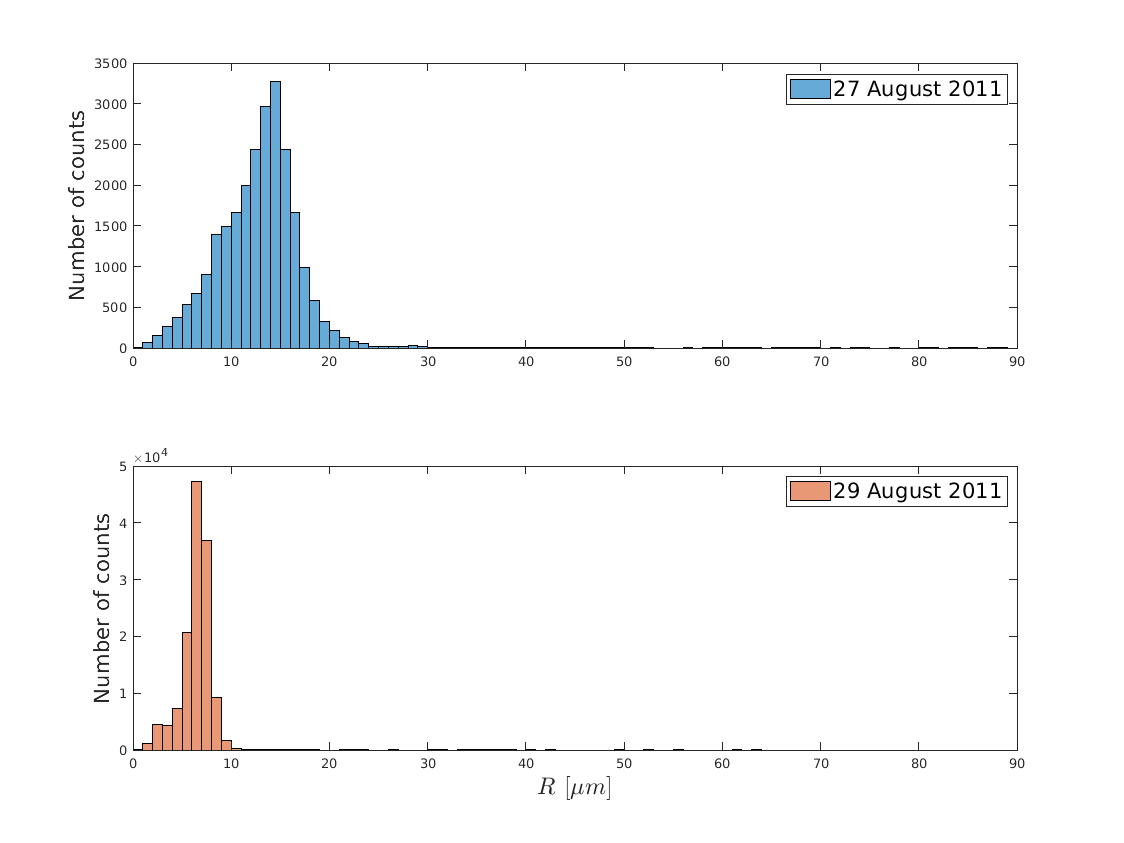
\includegraphics[width=30pc]{gfx/Hist_counts_raw.png}
\caption{Histograms of droplet size counts measured with a PDI probe at the UFS on 27th and 29th of August 2011.}
\label{fig:ch4_1}
\end{figure}

\begin{figure}[h]
\centering
\noindent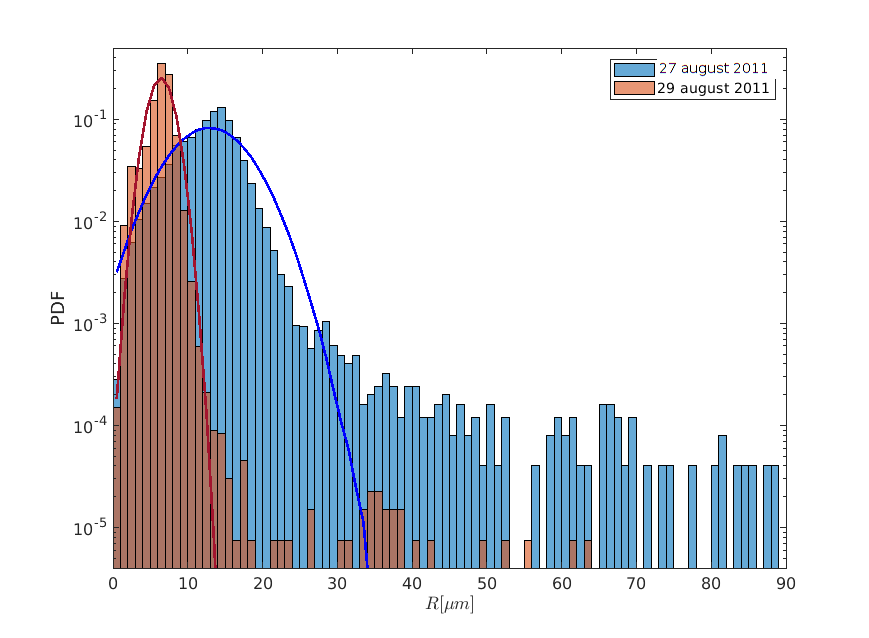
\includegraphics[width=30pc]{gfx/PDFs_log.png}
\caption{Droplet size probability distributions calculated for the data obtained with a PDI probe at the UFS on 27th and 29th of August 2011.}
\label{fig:ch4_2}
\end{figure}

High-resolution measurements of small-scale turbulence during cloud void events were conducted. Applying the methods described in Sec. \autoref{subs:atmosmeas}, mean energy dissipation rates and Kolmogorov scales were determined. Droplet and turbulence measured properties together with derived paremeters are summarized in Table \ref{tab:ch4_1}. Values of dimensionless parameters were calculated with the use of mean radius and Kolmogorov timescale. There is about one order of magnitude difference in $St$ between two cases, but the Froude numbers are comparable.

\begin{table}
\small
\tabcolsep=0.2cm
\caption{Properties of turbulence and cloud droplets during 30-minutes long observation periods. Values of dimensionless parameters are calculated with the use of mean radius.}
\centering
\begin{tabular}{|l|c|c|}
\hline
  & August 27th & August 29th\\
\hline
 Energy dissipation rate $\epsilon$ [cm$^2$/s$^3$] & 550 & 700 \\
\hline
 Kolmogorov length scale $\eta$ [mm] & 0.50  & 0.47\\
\hline
Komogorov timescale $\tau_{\eta}$ [ms] & 17 & 15\\
\hline
Droplet radius $R$ [$\mu$m] & 12.9 $\pm$ 4.8 & 6.4 $\pm$ 1.5\\
\hline
 Stokes number $St$ & 0.126  & 0.035\\
\hline
 Sedimentation parameter $S_v$ & 0.676  & 0.172\\
 \hline
 Froude number $Fr$ & 0.186  & 0.203\\
 \hline
 Number density $n$ [cm$^{-3}$] & 56 $\pm$ 47 & no data\\
 \hline
%\multicolumn{2}{l}{$^{a}$Footnote text here.}
\end{tabular}
\label{tab:ch4_1}
\end{table}

Multiple cloud images and movies were collected by laser-sheet imaging technique on the measurement days. In general two kinds of events in which droplet spatial distribution is visibly inhomogeneous were distinguished. The first kind is characterized by an irregular interface separating clear-air and cloudy-air volumes and/or cloudy volumes of visibly different properties over a wide range of spatial scales (panel b) in Fig. \ref{fig:ch4_3}). Inhomogeneities of the second kind, present within the cloudy volumes, were called cloud voids in ``Swiss cheese" clouds. Cloud voids were small (a few centimetres scale), the interface was usually blurry (see panels a) and c) in Fig. \ref{fig:ch4_3}) and the shapes of clear-air regions were often close to round or elliptic (see magnified voids in Fig. \ref{fig:ch4_4}). It is important to point out that the more intuitive expression "cloud holes" with regards to the second kind inhomogeneities is avoided on purpose because it is commonly used referring to the cloud-free regions occurring in stratocumulus decks, as described for example in \citet{Gerber_2005}.

\begin{figure}[h]
\centering
\noindent\includegraphics[width=35pc]{gfx/cloud_inhomog.png}
\caption{Examples of cloud voids observed at the UFS station with various camera-laser configurations. Images taken on 27 August (panel a) were chosen to estimate cloud void sizes. The ones recorded on 29 August evening (panel b) show the difference between inhomogeneities produced by cloud voids and those resulting from the mixing with clear air at the cloud edge. Other images from 29 August (panel c) suggest that the voids can be quite frequent in the sample volume. Bright spots and lines are due to presence of larger precipitation particles. 10~cm long segment is shown to represent spatial scale assumed in the void size calculation. For more details, see the movies attached in the supplementary materials.}
\label{fig:ch4_3}
\end{figure}

Inhomogeneities of the first kind are argued to be created in the process of cloud -- clear-air mixing (e.g. \cite{Warhaft_2000}). In contrast, in some series of images and movies, the shape of the recorded tracks of cloud droplets suggest the following cloud void origin hypothesis: they result from interactions between inertial, heavy cloud droplets and small-scale vortices present in a turbulent cloud. Comparison of the two described cases becomes straightforward when conducted on the basis of the enclosed movies \citep{database}. In the movie "ms01" between 13~s and 22~s there are two cloud void appearances. Motion of the void in the homogeneous cloud field resembles motion of a worm. Movie "ms02" presents cloudy and clear air mixing at the cloud edges. \\

\begin{figure}[h]
\centering
\noindent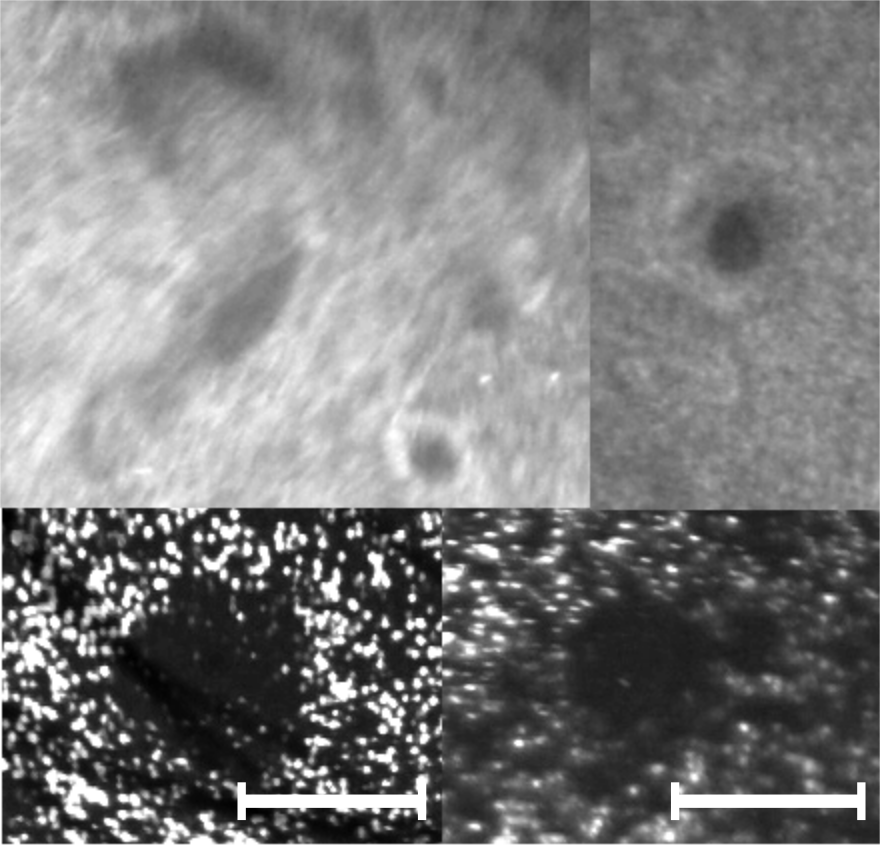
\includegraphics[width=35pc]{gfx/closeups.png}
\caption{Example close-ups of variously shaped cloud voids observed at the UFS station with different camera-laser configurations. 5~cm long section is placed in each image to represent spatial scale assumed in the void size calculation.}
\label{fig03}
\end{figure}

There were a few series of cloud void images collected with various laser-camera settings on the two experimental days. The best quality series, made in the morning of the 27th, was chosen for void size analysis. For the series of 17 photos selected for analysis, there were four in which voids were not clear enough to be accounted for. In the remaining 13 photos 27 voids were identified. Each one's size was manually determined. In the case of a round void, the diameter was taken as the size; in a case of flattened or ellipsoidal void, the maximal chord was taken. The typical void diameter was estimated to be 3.5$\pm$1~cm; the maximal, 12$\pm$4~cm; the minimal, 1$\pm$0.5~cm. Images from the analysed series from the morning of August 27th showing examples of objects identified as voids are presented in the panel a) of Fig. \ref{fig:ch4_3}. Voids captured on the 29th of August were not analysed due to the large uncertainty resulting from the unknown geometry of the camera-laser set-up. The general experimental observation was that the voids were smaller then those on August 27th. Definitive experimental verification of the cloud void origin is not possible on the basis of collected data only; however, in next sections, I argue that void creation due to inertia of droplets present inside vortex tubes is highly probable.

%------------------------------------------------
\section{Cloud void creation conditions}
\label{sec:void}
Using conclusions concerning the motion of a single particle, the following hypothesis on polydisperse particle collective behaviour can be formulated: a void can be created if a majority of the droplets have an unstable equilibrium point close to the axis $r^{\ast}_0<r^{\ast}_s$, leading to a limit cycle or periodic orbit attraction. The radius of curvature should be large enough for a void to be noticable. If multiple equilibrium points exist, attraction by a stable equilibrium point far from the axis $r^{\ast}_0>r^{\ast}_{min}$ should not considerably influence droplet trajectories close to the void considerably. The first and the last condition are inspected in the Subsect.\ref{ssec:poly}, the second  condition in the  Subsect.\ref{ssec:par}.

\subsection{Polydisperse particles motion analysis}
\label{ssec:poly}
Obtaining a mathematically strict condition for creation of an arbitrary sized void in arbitrary polydisperse collection of droplets would be too detailed and too complicated to be profitable for the interpretation of crude experimental results. Thorough analysis of single droplet motion in addition to what was presented in the paper \citep{Marcu_95}) was performed and used to draw approximate conclusions about polydisperse droplet motion.\\
The most obvious conclusion is that when circulation of the vortex is too small: $A \geq A_{cr}$,  the motion of particles is determined mostly by the gravitational force and resembles sedimentation through the vortex with curved trajectories. Circulation must then be large enough: at least $A \leq A_{cr}$ for void to be created.\\
The other condition is that equilibrium points near the vortex center for the majority of the particles are unstable, allowing circulation around the vortex axis. Inequality \ref{eq8} is exploited here to find the qualitative dependence between vortex and particle parameters that fulfills this condition.\\
First, distance from the vortex axis of the equilibrium point should be in the range $r^\ast \leq r^\ast_s$. It allows approximation of relation described by Eq. \ref{eq6} in the vicinity of $r^{\ast}=0$. The approximation is made with the assumption that in this vicinity the dependence on $A$ is weak (see Fig.2 in \citet{Marcu_95}).
%$r^{\ast}\simeq 4 \pi Sv$.
\begin{equation}
\left(\frac{Sv}{A}\right)^2=r^{\ast 2} \left[1+ \left( \frac{1-\exp \left(-r^{\ast 2}/2\right)}{2\pi Ar^{\ast 2}} \right)^2 \right]=r^{\ast 2}+\frac{(1-\exp \left(-r^{\ast 2}/2\right))^2}{(2\pi A r^{\ast})^2}\simeq r^{\ast 2}+\frac{1}{4 \pi^2 A^2} \frac{r^{\ast 2}}{4}=r^{\ast 2}\left( 1+(4 \pi A)^{-2}\right),
\label{eq10}
\end{equation}
 so in the end:
\begin{equation}
r^{\ast}_0\simeq 4 \pi Sv \left(1+(4\pi A)^2\right)^{-\frac{1}{2}}.
\label{eq11}
\end{equation}

Secondly, the function $\phi(r^\ast_0)$ (see Fig.3 in \citet{Marcu_95}) is approximated in the chosen $r^\ast$ range  by linear dependence on $r^\ast$ : ${\phi(r^\ast_0)\simeq-\left(1-r^\ast_0/r^\ast_s \right)\cdot\left(16 \pi^2\right)^{-1}}$. At $r^{\ast}=0$ it has the same form as obtained for the case without gravity in \citet{Marcu_95}. 
\noindent The above approximations are used simplifying the stability condition determined by Eq. \ref{eq8}. In the end the condition for unstable points near the axis are algebraicly transformed and expressed by spliting it in two parts. The first part concerns only the vortex parameters and the second part the particle sizes.\\

The first part requires that strain parameter $A$ is small enough:
\begin{equation}
A < A_{max} \propto B^{1/3}
\label{eq12}
\end{equation}
and consequently circulation $\Gamma$ large enough:
\begin{equation}
\Gamma > \Gamma_{min} \propto B^{-1/3}
\label{eq13}
\end{equation}
\noindent The second part demands that particle Stokes number falls within the range $(St_1,St_1+\Delta St)$ and it is related to the vortex parameters (results shown to the leading term order in $A$):
\begin{equation}
\begin{array}{l}
St_1 \propto A  \\
\Delta St \propto B A^{-2}
\end{array} .
\label{eq14}
\end{equation}

\noindent $B$ is a new dimensionless parameter depending on vortex core size $\delta$ and gravity influence $g sin\theta$:
\begin{equation}
B=\underbrace{\frac{r^{\ast}_s}{2^8 \pi^3}}_{const} \frac{\nu^2}{g \sin\theta \delta^3}.
\label{eq15}
\end{equation}
\noindent The maximal strain parameter $A_{max}$ (minimal circulation $\Gamma_{min}$) increases (decreases) weakly with $B$. So the larger the vortex core size $\delta$ and gravity influence $g sin\theta$ the larger the minimal circulation needed.

\noindent The following conclusions can be drawn from the above approximate relations:

\begin{itemize}
\item There is a threshold (minimal) value of circulation needed for void creation. It increases with inclination angle ($\sin \theta$) and vortex size $\delta$.
\item The greater the circulation the smaller particles  have their unstable points near the axis.
\item The range of particles having unstable points near the axis increases with increasing circulation and decreases with increasing gravity influence and vortex size $\delta$.
\end{itemize}

\noindent Building up on these results it may be concluded that it is harder to observe voids created by horizontally aligned vortices than vertically aligned ones and also more difficult to observe voids the larger particle size range is.\\

\subsection{Particle orbit in a void - the radius of curvature}
\label{ssec:par}
In order to obtain a void, a majority of the droplets must circle around the axis and the curvature of their trajectories should be large enough for a void to be noticable. In order to estimate the curvature radius we perform the following reasoning. For simplicity particle and vortex constants and parameters are now chosen to match those of water droplets in the cloudy air and henceforward particles are called droplets.
Firstly, a basic vortex spatial scale is established for the measurement conditions. Premises found in the literature discussed in the introduction were used for making the assumption that the proportionality constant in Eq. \ref{eq1} is in the range $m\in[3.5, 24]$. It means $\delta \in [0.18,1.20]$~cm for August 27th measurements.
Secondly, the droplet trajectory curvature radius is approximated by the periodic orbit radius which is a solution of Eq. \ref{eq5}. For this reason, solutions of Eq.\ref{eq5} are presented in Fig.\ref{fig05} for various representative vortex parameters. Every color represents one of droplet sizes: $R=3,13,23$~$\mu m$ chosen to be within the experimental range for August 27th (see Table \ref{tab01}). Overlapping colored surfaces match regions in which solutions can exist (what corresponds to the condition $St<St_{cr}$). Dashed lines are contour plots of solutions of chosen (close to experimental) void sizes: 0.5~cm, 1.5~cm, 3~cm. Using the information presented in this plot, the analysed strain parameter was further limited, from $A<A_{cr}$ down to $A \in [10^{-4}, 8\cdot10^{-3}]$.

\begin{figure*}
\centering
\noindent 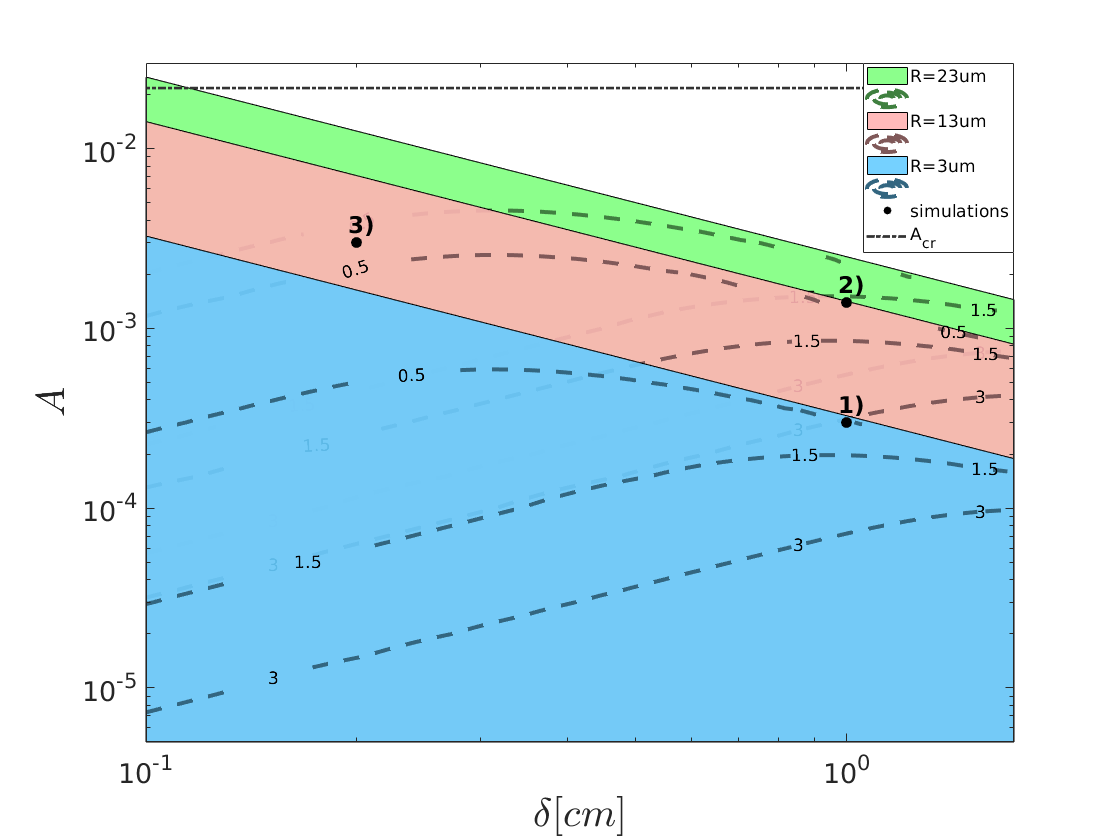
\includegraphics[width=30pc]{gfx/fig05.png}
\caption{ Contour plot of stable periodic 2D orbit radius for droplets of radii $R=3,13,23 \ \mu m$ covering the experimental range on August 27th. Selected ranges of vortex parameters: vortex core size $\delta$ and strain $A$ are in x an y axes, respectively. Overlapping (blue on a top, then pink and green) colored surfaces match subspaces in which stable periodic 2D orbit exist for droplet radius given by its colour. Dashed lines are contour plots of solutions of chosen void sizes:0.5~cm ,1.5~cm, 3~cm. Black points represent parameters set for simulations as described in Sect.\ref{sec:Mie}.}
\label{fig05}
\end{figure*}

\subsection{Timescales of motion}
%------------------------------------------------

\end{document}